\documentclass{article}

\usepackage[margin=0.8in]{geometry}
\usepackage{amsmath, amsfonts}
\usepackage{booktabs}
\usepackage{hyperref}
\usepackage{xcolor}
\usepackage{tikz}
\usepackage{graphicx}

\tikzset{block/.style ={rectangle,draw}
}
\usetikzlibrary{positioning, shapes.geometric}
\usetikzlibrary{trees}

\setlength{\parindent}{0pt}

\begin{document}

\section*{EVB Decomposition}
Change in the value function due to learning after taking action $a^*$:

\begin{align}
v(ba^*)-v(b)=&\sum_{b'}p(b'\mid b, a^*)\Big(v(b')-v(b)\Big)\\
=&\sum_{b'}p(b'\mid b, a^*)\Big(\sum_a \pi(a\mid b')q(b', a)-\sum_{a} \pi(a\mid b)q(b,a)\Big) \nonumber \\
=&\sum_{b'}p(b'\mid b, a^*)\sum_a\Big(\big(\pi(a\mid b')-\pi(a\mid b)\big)q(b',a) \nonumber \\
+&\pi(a\mid b)\big(q(b', a) - q(b, a)\big)\Big) \nonumber
\end{align}

Expanding $q(b', a) - q(b, a)$:

\begin{align}
q(b', a)-q(b, a)=&\sum_{b''}p(b''\mid b', a)\big[r(b',a) + \gamma v(b'')\big]\\
-&\sum_{b'}p(g'\mid b, a)\big[r(b,a) + \gamma v(g')\big]\nonumber\\
=& r(b',a) + \gamma \sum_{b''}p(b''\mid b', a)v(b'')\nonumber \\
-& r(b,a) + \gamma \sum_{g'}p(g'\mid b, a)v(g')\nonumber \\
=& \underbrace{\vphantom{ \left(\frac{a^{\frac{0.3}{`}}}{b}\right)} r(b',a) - r(b,a)}_{\substack{\text{Difference in the expected} \\ \text{immediate return}}} + \underbrace{\gamma \big[ \sum_{b''}p(b''\mid b', a)v(b'') - \sum_{g'}p(g'\mid b, a)v(g') \big]}_{\substack{\text{Difference in the expected} \\ \text{future return}}}\nonumber
\end{align}

So overall the EVB decomposes as:

\begin{align}
    v(ba^*)-v(b) =& \mathbb{E}_{b'\sim p(b'\mid b, a^*)}\Big[\sum_a \big(\pi(a\mid b')-\pi(a\mid b)\big)q(b',a) \\
    +& \mathbb{E}_{a\sim \pi(a\mid b)}\big[r(b',a) - r(b,a)\big] \nonumber \\ 
    +& \mathbb{E}_{a\sim \pi(a\mid b)}\big[\gamma \sum_{b''}p(b''\mid b', a)v(b'') - \gamma \sum_{g'}p(g'\mid b, a)v(g') \big] \Big] \nonumber
\end{align}

One last thing to consider is how the prioritisation of distal experiences should 
differ from those that are more immediate. This also has implications for how likely 
those experiences are to occur according to the current model. 
\bigbreak
For instance, if the agent considers updating $v(b)$ towards the value that would result 
from taking a particular action from that belief state -- say, $v(ba^*)$ -- the EVB associated 
with that update needs to be weighted by the probability of transitioning into 
belief state $b$ in the first place (i.e., from the current root of the tree).

\begin{align}
    v(ba^*)-v(b) = p(b_{\text{root}}\rightarrow b) \times  
    \Big(&\mathbb{E}_{b'\sim p(b'\mid b, a^*)}\Big[\sum_a \big(\pi(a\mid b')-\pi(a\mid b)\big)q(b',a) \\
    +& \mathbb{E}_{a\sim \pi(a\mid b)}\big[r(b',a) - r(b,a)\big] \nonumber \\ 
    +& \mathbb{E}_{a\sim \pi(a\mid b)}\big[\gamma \sum_{b''}p(b''\mid b', a)v(b'') - \gamma \sum_{g'}p(g'\mid b, a)v(g') \big] \Big] \Big) \nonumber
\end{align}

\newpage
\section*{Simulations}

Prioritisation pattern with horizon $h=2$. Each orange box is a belief state, and 
the parameters that correspond to that belief are written inside. Red arrows show 
which replay updates were executed.
\vspace{1cm}

\input{../Data/Tree/tex_tree_small.tex}

\newpage
Prioritisation pattern with horizon $h=4$. The prior belief at the root is set to the 
same values as in the above example with shorter horizon. Note that for this (and the 
previous) tree, EVB was not scaled by the probability of reaching any belief.
\vspace{1cm}

\input{../Data/Tree/tex_tree_big.tex}

\newpage
Prioritisation pattern with horizon $h=4$. Same example as before, however, here, each 
EVB value $v(ba^*)-v(b)$ is scaled by the probability of reaching belief $b$ from the root 
of the tree. Note how the less-likely branches are ignored in this case, as opposed to the 
one showed above.
\vspace{1cm}

\begin{minipage}{\textwidth}
\centering
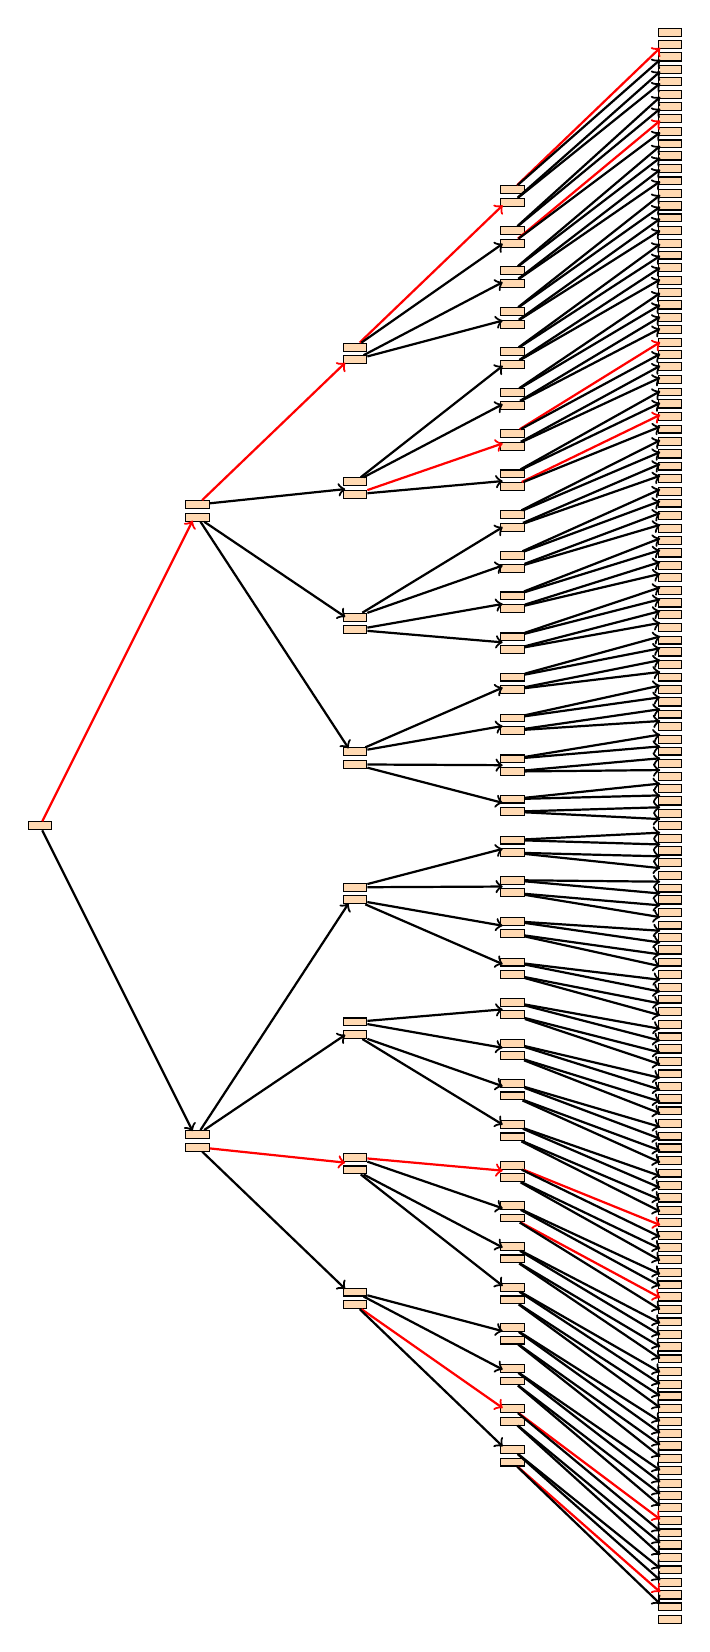
\begin{tikzpicture}
\tikzstyle{between} = [rectangle, draw=none]
\tikzstyle{state}   = [rectangle, text centered, draw=black, minimum height=1mm, text width=3mm, inner sep=0pt, fill=orange!30]
\node[between] at (-7.00, 4.00) (1_b_0){};
\node[between] at (-7.00, -4.00) (1_b_1){};
\node[between] at (-5.00, 6.00) (2_b_0){};
\node[between] at (-5.00, 4.29) (2_b_1){};
\node[between] at (-5.00, 2.57) (2_b_2){};
\node[between] at (-5.00, 0.86) (2_b_3){};
\node[between] at (-5.00, -0.86) (2_b_4){};
\node[between] at (-5.00, -2.57) (2_b_5){};
\node[between] at (-5.00, -4.29) (2_b_6){};
\node[between] at (-5.00, -6.00) (2_b_7){};
\node[between] at (-3.00, 8.00) (3_b_0){};
\node[between] at (-3.00, 7.48) (3_b_1){};
\node[between] at (-3.00, 6.97) (3_b_2){};
\node[between] at (-3.00, 6.45) (3_b_3){};
\node[between] at (-3.00, 5.94) (3_b_4){};
\node[between] at (-3.00, 5.42) (3_b_5){};
\node[between] at (-3.00, 4.90) (3_b_6){};
\node[between] at (-3.00, 4.39) (3_b_7){};
\node[between] at (-3.00, 3.87) (3_b_8){};
\node[between] at (-3.00, 3.35) (3_b_9){};
\node[between] at (-3.00, 2.84) (3_b_10){};
\node[between] at (-3.00, 2.32) (3_b_11){};
\node[between] at (-3.00, 1.81) (3_b_12){};
\node[between] at (-3.00, 1.29) (3_b_13){};
\node[between] at (-3.00, 0.77) (3_b_14){};
\node[between] at (-3.00, 0.26) (3_b_15){};
\node[between] at (-3.00, -0.26) (3_b_16){};
\node[between] at (-3.00, -0.77) (3_b_17){};
\node[between] at (-3.00, -1.29) (3_b_18){};
\node[between] at (-3.00, -1.81) (3_b_19){};
\node[between] at (-3.00, -2.32) (3_b_20){};
\node[between] at (-3.00, -2.84) (3_b_21){};
\node[between] at (-3.00, -3.35) (3_b_22){};
\node[between] at (-3.00, -3.87) (3_b_23){};
\node[between] at (-3.00, -4.39) (3_b_24){};
\node[between] at (-3.00, -4.90) (3_b_25){};
\node[between] at (-3.00, -5.42) (3_b_26){};
\node[between] at (-3.00, -5.94) (3_b_27){};
\node[between] at (-3.00, -6.45) (3_b_28){};
\node[between] at (-3.00, -6.97) (3_b_29){};
\node[between] at (-3.00, -7.48) (3_b_30){};
\node[between] at (-3.00, -8.00) (3_b_31){};
\node[between] at (-1.00, 10.00) (4_b_0){};
\node[between] at (-1.00, 9.84) (4_b_1){};
\node[between] at (-1.00, 9.69) (4_b_2){};
\node[between] at (-1.00, 9.53) (4_b_3){};
\node[between] at (-1.00, 9.37) (4_b_4){};
\node[between] at (-1.00, 9.21) (4_b_5){};
\node[between] at (-1.00, 9.06) (4_b_6){};
\node[between] at (-1.00, 8.90) (4_b_7){};
\node[between] at (-1.00, 8.74) (4_b_8){};
\node[between] at (-1.00, 8.58) (4_b_9){};
\node[between] at (-1.00, 8.43) (4_b_10){};
\node[between] at (-1.00, 8.27) (4_b_11){};
\node[between] at (-1.00, 8.11) (4_b_12){};
\node[between] at (-1.00, 7.95) (4_b_13){};
\node[between] at (-1.00, 7.80) (4_b_14){};
\node[between] at (-1.00, 7.64) (4_b_15){};
\node[between] at (-1.00, 7.48) (4_b_16){};
\node[between] at (-1.00, 7.32) (4_b_17){};
\node[between] at (-1.00, 7.17) (4_b_18){};
\node[between] at (-1.00, 7.01) (4_b_19){};
\node[between] at (-1.00, 6.85) (4_b_20){};
\node[between] at (-1.00, 6.69) (4_b_21){};
\node[between] at (-1.00, 6.54) (4_b_22){};
\node[between] at (-1.00, 6.38) (4_b_23){};
\node[between] at (-1.00, 6.22) (4_b_24){};
\node[between] at (-1.00, 6.06) (4_b_25){};
\node[between] at (-1.00, 5.91) (4_b_26){};
\node[between] at (-1.00, 5.75) (4_b_27){};
\node[between] at (-1.00, 5.59) (4_b_28){};
\node[between] at (-1.00, 5.43) (4_b_29){};
\node[between] at (-1.00, 5.28) (4_b_30){};
\node[between] at (-1.00, 5.12) (4_b_31){};
\node[between] at (-1.00, 4.96) (4_b_32){};
\node[between] at (-1.00, 4.80) (4_b_33){};
\node[between] at (-1.00, 4.65) (4_b_34){};
\node[between] at (-1.00, 4.49) (4_b_35){};
\node[between] at (-1.00, 4.33) (4_b_36){};
\node[between] at (-1.00, 4.17) (4_b_37){};
\node[between] at (-1.00, 4.02) (4_b_38){};
\node[between] at (-1.00, 3.86) (4_b_39){};
\node[between] at (-1.00, 3.70) (4_b_40){};
\node[between] at (-1.00, 3.54) (4_b_41){};
\node[between] at (-1.00, 3.39) (4_b_42){};
\node[between] at (-1.00, 3.23) (4_b_43){};
\node[between] at (-1.00, 3.07) (4_b_44){};
\node[between] at (-1.00, 2.91) (4_b_45){};
\node[between] at (-1.00, 2.76) (4_b_46){};
\node[between] at (-1.00, 2.60) (4_b_47){};
\node[between] at (-1.00, 2.44) (4_b_48){};
\node[between] at (-1.00, 2.28) (4_b_49){};
\node[between] at (-1.00, 2.13) (4_b_50){};
\node[between] at (-1.00, 1.97) (4_b_51){};
\node[between] at (-1.00, 1.81) (4_b_52){};
\node[between] at (-1.00, 1.65) (4_b_53){};
\node[between] at (-1.00, 1.50) (4_b_54){};
\node[between] at (-1.00, 1.34) (4_b_55){};
\node[between] at (-1.00, 1.18) (4_b_56){};
\node[between] at (-1.00, 1.02) (4_b_57){};
\node[between] at (-1.00, 0.87) (4_b_58){};
\node[between] at (-1.00, 0.71) (4_b_59){};
\node[between] at (-1.00, 0.55) (4_b_60){};
\node[between] at (-1.00, 0.39) (4_b_61){};
\node[between] at (-1.00, 0.24) (4_b_62){};
\node[between] at (-1.00, 0.08) (4_b_63){};
\node[between] at (-1.00, -0.08) (4_b_64){};
\node[between] at (-1.00, -0.24) (4_b_65){};
\node[between] at (-1.00, -0.39) (4_b_66){};
\node[between] at (-1.00, -0.55) (4_b_67){};
\node[between] at (-1.00, -0.71) (4_b_68){};
\node[between] at (-1.00, -0.87) (4_b_69){};
\node[between] at (-1.00, -1.02) (4_b_70){};
\node[between] at (-1.00, -1.18) (4_b_71){};
\node[between] at (-1.00, -1.34) (4_b_72){};
\node[between] at (-1.00, -1.50) (4_b_73){};
\node[between] at (-1.00, -1.65) (4_b_74){};
\node[between] at (-1.00, -1.81) (4_b_75){};
\node[between] at (-1.00, -1.97) (4_b_76){};
\node[between] at (-1.00, -2.13) (4_b_77){};
\node[between] at (-1.00, -2.28) (4_b_78){};
\node[between] at (-1.00, -2.44) (4_b_79){};
\node[between] at (-1.00, -2.60) (4_b_80){};
\node[between] at (-1.00, -2.76) (4_b_81){};
\node[between] at (-1.00, -2.91) (4_b_82){};
\node[between] at (-1.00, -3.07) (4_b_83){};
\node[between] at (-1.00, -3.23) (4_b_84){};
\node[between] at (-1.00, -3.39) (4_b_85){};
\node[between] at (-1.00, -3.54) (4_b_86){};
\node[between] at (-1.00, -3.70) (4_b_87){};
\node[between] at (-1.00, -3.86) (4_b_88){};
\node[between] at (-1.00, -4.02) (4_b_89){};
\node[between] at (-1.00, -4.17) (4_b_90){};
\node[between] at (-1.00, -4.33) (4_b_91){};
\node[between] at (-1.00, -4.49) (4_b_92){};
\node[between] at (-1.00, -4.65) (4_b_93){};
\node[between] at (-1.00, -4.80) (4_b_94){};
\node[between] at (-1.00, -4.96) (4_b_95){};
\node[between] at (-1.00, -5.12) (4_b_96){};
\node[between] at (-1.00, -5.28) (4_b_97){};
\node[between] at (-1.00, -5.43) (4_b_98){};
\node[between] at (-1.00, -5.59) (4_b_99){};
\node[between] at (-1.00, -5.75) (4_b_100){};
\node[between] at (-1.00, -5.91) (4_b_101){};
\node[between] at (-1.00, -6.06) (4_b_102){};
\node[between] at (-1.00, -6.22) (4_b_103){};
\node[between] at (-1.00, -6.38) (4_b_104){};
\node[between] at (-1.00, -6.54) (4_b_105){};
\node[between] at (-1.00, -6.69) (4_b_106){};
\node[between] at (-1.00, -6.85) (4_b_107){};
\node[between] at (-1.00, -7.01) (4_b_108){};
\node[between] at (-1.00, -7.17) (4_b_109){};
\node[between] at (-1.00, -7.32) (4_b_110){};
\node[between] at (-1.00, -7.48) (4_b_111){};
\node[between] at (-1.00, -7.64) (4_b_112){};
\node[between] at (-1.00, -7.80) (4_b_113){};
\node[between] at (-1.00, -7.95) (4_b_114){};
\node[between] at (-1.00, -8.11) (4_b_115){};
\node[between] at (-1.00, -8.27) (4_b_116){};
\node[between] at (-1.00, -8.43) (4_b_117){};
\node[between] at (-1.00, -8.58) (4_b_118){};
\node[between] at (-1.00, -8.74) (4_b_119){};
\node[between] at (-1.00, -8.90) (4_b_120){};
\node[between] at (-1.00, -9.06) (4_b_121){};
\node[between] at (-1.00, -9.21) (4_b_122){};
\node[between] at (-1.00, -9.37) (4_b_123){};
\node[between] at (-1.00, -9.53) (4_b_124){};
\node[between] at (-1.00, -9.69) (4_b_125){};
\node[between] at (-1.00, -9.84) (4_b_126){};
\node[between] at (-1.00, -10.00) (4_b_127){};
\node[state] at (-9.00, 0.00) (0_s_0){};
\node[state] at (-7.00, 4.08) (1_s_0){};
\node[state] at (-7.00, 3.92) (1_s_1){};
\node[state] at (-7.00, -3.92) (1_s_2){};
\node[state] at (-7.00, -4.08) (1_s_3){};
\node[state] at (-5.00, 6.08) (2_s_0){};
\node[state] at (-5.00, 5.92) (2_s_1){};
\node[state] at (-5.00, 4.37) (2_s_2){};
\node[state] at (-5.00, 4.21) (2_s_3){};
\node[state] at (-5.00, 2.65) (2_s_4){};
\node[state] at (-5.00, 2.49) (2_s_5){};
\node[state] at (-5.00, 0.94) (2_s_6){};
\node[state] at (-5.00, 0.78) (2_s_7){};
\node[state] at (-5.00, -0.78) (2_s_8){};
\node[state] at (-5.00, -0.94) (2_s_9){};
\node[state] at (-5.00, -2.49) (2_s_10){};
\node[state] at (-5.00, -2.65) (2_s_11){};
\node[state] at (-5.00, -4.21) (2_s_12){};
\node[state] at (-5.00, -4.37) (2_s_13){};
\node[state] at (-5.00, -5.92) (2_s_14){};
\node[state] at (-5.00, -6.08) (2_s_15){};
\node[state] at (-3.00, 8.08) (3_s_0){};
\node[state] at (-3.00, 7.92) (3_s_1){};
\node[state] at (-3.00, 7.56) (3_s_2){};
\node[state] at (-3.00, 7.40) (3_s_3){};
\node[state] at (-3.00, 7.05) (3_s_4){};
\node[state] at (-3.00, 6.89) (3_s_5){};
\node[state] at (-3.00, 6.53) (3_s_6){};
\node[state] at (-3.00, 6.37) (3_s_7){};
\node[state] at (-3.00, 6.02) (3_s_8){};
\node[state] at (-3.00, 5.86) (3_s_9){};
\node[state] at (-3.00, 5.50) (3_s_10){};
\node[state] at (-3.00, 5.34) (3_s_11){};
\node[state] at (-3.00, 4.98) (3_s_12){};
\node[state] at (-3.00, 4.82) (3_s_13){};
\node[state] at (-3.00, 4.47) (3_s_14){};
\node[state] at (-3.00, 4.31) (3_s_15){};
\node[state] at (-3.00, 3.95) (3_s_16){};
\node[state] at (-3.00, 3.79) (3_s_17){};
\node[state] at (-3.00, 3.43) (3_s_18){};
\node[state] at (-3.00, 3.27) (3_s_19){};
\node[state] at (-3.00, 2.92) (3_s_20){};
\node[state] at (-3.00, 2.76) (3_s_21){};
\node[state] at (-3.00, 2.40) (3_s_22){};
\node[state] at (-3.00, 2.24) (3_s_23){};
\node[state] at (-3.00, 1.89) (3_s_24){};
\node[state] at (-3.00, 1.73) (3_s_25){};
\node[state] at (-3.00, 1.37) (3_s_26){};
\node[state] at (-3.00, 1.21) (3_s_27){};
\node[state] at (-3.00, 0.85) (3_s_28){};
\node[state] at (-3.00, 0.69) (3_s_29){};
\node[state] at (-3.00, 0.34) (3_s_30){};
\node[state] at (-3.00, 0.18) (3_s_31){};
\node[state] at (-3.00, -0.18) (3_s_32){};
\node[state] at (-3.00, -0.34) (3_s_33){};
\node[state] at (-3.00, -0.69) (3_s_34){};
\node[state] at (-3.00, -0.85) (3_s_35){};
\node[state] at (-3.00, -1.21) (3_s_36){};
\node[state] at (-3.00, -1.37) (3_s_37){};
\node[state] at (-3.00, -1.73) (3_s_38){};
\node[state] at (-3.00, -1.89) (3_s_39){};
\node[state] at (-3.00, -2.24) (3_s_40){};
\node[state] at (-3.00, -2.40) (3_s_41){};
\node[state] at (-3.00, -2.76) (3_s_42){};
\node[state] at (-3.00, -2.92) (3_s_43){};
\node[state] at (-3.00, -3.27) (3_s_44){};
\node[state] at (-3.00, -3.43) (3_s_45){};
\node[state] at (-3.00, -3.79) (3_s_46){};
\node[state] at (-3.00, -3.95) (3_s_47){};
\node[state] at (-3.00, -4.31) (3_s_48){};
\node[state] at (-3.00, -4.47) (3_s_49){};
\node[state] at (-3.00, -4.82) (3_s_50){};
\node[state] at (-3.00, -4.98) (3_s_51){};
\node[state] at (-3.00, -5.34) (3_s_52){};
\node[state] at (-3.00, -5.50) (3_s_53){};
\node[state] at (-3.00, -5.86) (3_s_54){};
\node[state] at (-3.00, -6.02) (3_s_55){};
\node[state] at (-3.00, -6.37) (3_s_56){};
\node[state] at (-3.00, -6.53) (3_s_57){};
\node[state] at (-3.00, -6.89) (3_s_58){};
\node[state] at (-3.00, -7.05) (3_s_59){};
\node[state] at (-3.00, -7.40) (3_s_60){};
\node[state] at (-3.00, -7.56) (3_s_61){};
\node[state] at (-3.00, -7.92) (3_s_62){};
\node[state] at (-3.00, -8.08) (3_s_63){};
\node[state] at (-1.00, 10.08) (4_s_0){};
\node[state] at (-1.00, 9.92) (4_s_1){};
\node[state] at (-1.00, 9.92) (4_s_2){};
\node[state] at (-1.00, 9.76) (4_s_3){};
\node[state] at (-1.00, 9.77) (4_s_4){};
\node[state] at (-1.00, 9.61) (4_s_5){};
\node[state] at (-1.00, 9.61) (4_s_6){};
\node[state] at (-1.00, 9.45) (4_s_7){};
\node[state] at (-1.00, 9.45) (4_s_8){};
\node[state] at (-1.00, 9.29) (4_s_9){};
\node[state] at (-1.00, 9.29) (4_s_10){};
\node[state] at (-1.00, 9.13) (4_s_11){};
\node[state] at (-1.00, 9.14) (4_s_12){};
\node[state] at (-1.00, 8.98) (4_s_13){};
\node[state] at (-1.00, 8.98) (4_s_14){};
\node[state] at (-1.00, 8.82) (4_s_15){};
\node[state] at (-1.00, 8.82) (4_s_16){};
\node[state] at (-1.00, 8.66) (4_s_17){};
\node[state] at (-1.00, 8.66) (4_s_18){};
\node[state] at (-1.00, 8.50) (4_s_19){};
\node[state] at (-1.00, 8.51) (4_s_20){};
\node[state] at (-1.00, 8.35) (4_s_21){};
\node[state] at (-1.00, 8.35) (4_s_22){};
\node[state] at (-1.00, 8.19) (4_s_23){};
\node[state] at (-1.00, 8.19) (4_s_24){};
\node[state] at (-1.00, 8.03) (4_s_25){};
\node[state] at (-1.00, 8.03) (4_s_26){};
\node[state] at (-1.00, 7.87) (4_s_27){};
\node[state] at (-1.00, 7.88) (4_s_28){};
\node[state] at (-1.00, 7.72) (4_s_29){};
\node[state] at (-1.00, 7.72) (4_s_30){};
\node[state] at (-1.00, 7.56) (4_s_31){};
\node[state] at (-1.00, 7.56) (4_s_32){};
\node[state] at (-1.00, 7.40) (4_s_33){};
\node[state] at (-1.00, 7.40) (4_s_34){};
\node[state] at (-1.00, 7.24) (4_s_35){};
\node[state] at (-1.00, 7.25) (4_s_36){};
\node[state] at (-1.00, 7.09) (4_s_37){};
\node[state] at (-1.00, 7.09) (4_s_38){};
\node[state] at (-1.00, 6.93) (4_s_39){};
\node[state] at (-1.00, 6.93) (4_s_40){};
\node[state] at (-1.00, 6.77) (4_s_41){};
\node[state] at (-1.00, 6.77) (4_s_42){};
\node[state] at (-1.00, 6.61) (4_s_43){};
\node[state] at (-1.00, 6.62) (4_s_44){};
\node[state] at (-1.00, 6.46) (4_s_45){};
\node[state] at (-1.00, 6.46) (4_s_46){};
\node[state] at (-1.00, 6.30) (4_s_47){};
\node[state] at (-1.00, 6.30) (4_s_48){};
\node[state] at (-1.00, 6.14) (4_s_49){};
\node[state] at (-1.00, 6.14) (4_s_50){};
\node[state] at (-1.00, 5.98) (4_s_51){};
\node[state] at (-1.00, 5.99) (4_s_52){};
\node[state] at (-1.00, 5.83) (4_s_53){};
\node[state] at (-1.00, 5.83) (4_s_54){};
\node[state] at (-1.00, 5.67) (4_s_55){};
\node[state] at (-1.00, 5.67) (4_s_56){};
\node[state] at (-1.00, 5.51) (4_s_57){};
\node[state] at (-1.00, 5.51) (4_s_58){};
\node[state] at (-1.00, 5.35) (4_s_59){};
\node[state] at (-1.00, 5.36) (4_s_60){};
\node[state] at (-1.00, 5.20) (4_s_61){};
\node[state] at (-1.00, 5.20) (4_s_62){};
\node[state] at (-1.00, 5.04) (4_s_63){};
\node[state] at (-1.00, 5.04) (4_s_64){};
\node[state] at (-1.00, 4.88) (4_s_65){};
\node[state] at (-1.00, 4.88) (4_s_66){};
\node[state] at (-1.00, 4.72) (4_s_67){};
\node[state] at (-1.00, 4.73) (4_s_68){};
\node[state] at (-1.00, 4.57) (4_s_69){};
\node[state] at (-1.00, 4.57) (4_s_70){};
\node[state] at (-1.00, 4.41) (4_s_71){};
\node[state] at (-1.00, 4.41) (4_s_72){};
\node[state] at (-1.00, 4.25) (4_s_73){};
\node[state] at (-1.00, 4.25) (4_s_74){};
\node[state] at (-1.00, 4.09) (4_s_75){};
\node[state] at (-1.00, 4.10) (4_s_76){};
\node[state] at (-1.00, 3.94) (4_s_77){};
\node[state] at (-1.00, 3.94) (4_s_78){};
\node[state] at (-1.00, 3.78) (4_s_79){};
\node[state] at (-1.00, 3.78) (4_s_80){};
\node[state] at (-1.00, 3.62) (4_s_81){};
\node[state] at (-1.00, 3.62) (4_s_82){};
\node[state] at (-1.00, 3.46) (4_s_83){};
\node[state] at (-1.00, 3.47) (4_s_84){};
\node[state] at (-1.00, 3.31) (4_s_85){};
\node[state] at (-1.00, 3.31) (4_s_86){};
\node[state] at (-1.00, 3.15) (4_s_87){};
\node[state] at (-1.00, 3.15) (4_s_88){};
\node[state] at (-1.00, 2.99) (4_s_89){};
\node[state] at (-1.00, 2.99) (4_s_90){};
\node[state] at (-1.00, 2.83) (4_s_91){};
\node[state] at (-1.00, 2.84) (4_s_92){};
\node[state] at (-1.00, 2.68) (4_s_93){};
\node[state] at (-1.00, 2.68) (4_s_94){};
\node[state] at (-1.00, 2.52) (4_s_95){};
\node[state] at (-1.00, 2.52) (4_s_96){};
\node[state] at (-1.00, 2.36) (4_s_97){};
\node[state] at (-1.00, 2.36) (4_s_98){};
\node[state] at (-1.00, 2.20) (4_s_99){};
\node[state] at (-1.00, 2.21) (4_s_100){};
\node[state] at (-1.00, 2.05) (4_s_101){};
\node[state] at (-1.00, 2.05) (4_s_102){};
\node[state] at (-1.00, 1.89) (4_s_103){};
\node[state] at (-1.00, 1.89) (4_s_104){};
\node[state] at (-1.00, 1.73) (4_s_105){};
\node[state] at (-1.00, 1.73) (4_s_106){};
\node[state] at (-1.00, 1.57) (4_s_107){};
\node[state] at (-1.00, 1.58) (4_s_108){};
\node[state] at (-1.00, 1.42) (4_s_109){};
\node[state] at (-1.00, 1.42) (4_s_110){};
\node[state] at (-1.00, 1.26) (4_s_111){};
\node[state] at (-1.00, 1.26) (4_s_112){};
\node[state] at (-1.00, 1.10) (4_s_113){};
\node[state] at (-1.00, 1.10) (4_s_114){};
\node[state] at (-1.00, 0.94) (4_s_115){};
\node[state] at (-1.00, 0.95) (4_s_116){};
\node[state] at (-1.00, 0.79) (4_s_117){};
\node[state] at (-1.00, 0.79) (4_s_118){};
\node[state] at (-1.00, 0.63) (4_s_119){};
\node[state] at (-1.00, 0.63) (4_s_120){};
\node[state] at (-1.00, 0.47) (4_s_121){};
\node[state] at (-1.00, 0.47) (4_s_122){};
\node[state] at (-1.00, 0.31) (4_s_123){};
\node[state] at (-1.00, 0.32) (4_s_124){};
\node[state] at (-1.00, 0.16) (4_s_125){};
\node[state] at (-1.00, 0.16) (4_s_126){};
\node[state] at (-1.00, -0.00) (4_s_127){};
\node[state] at (-1.00, 0.00) (4_s_128){};
\node[state] at (-1.00, -0.16) (4_s_129){};
\node[state] at (-1.00, -0.16) (4_s_130){};
\node[state] at (-1.00, -0.32) (4_s_131){};
\node[state] at (-1.00, -0.31) (4_s_132){};
\node[state] at (-1.00, -0.47) (4_s_133){};
\node[state] at (-1.00, -0.47) (4_s_134){};
\node[state] at (-1.00, -0.63) (4_s_135){};
\node[state] at (-1.00, -0.63) (4_s_136){};
\node[state] at (-1.00, -0.79) (4_s_137){};
\node[state] at (-1.00, -0.79) (4_s_138){};
\node[state] at (-1.00, -0.95) (4_s_139){};
\node[state] at (-1.00, -0.94) (4_s_140){};
\node[state] at (-1.00, -1.10) (4_s_141){};
\node[state] at (-1.00, -1.10) (4_s_142){};
\node[state] at (-1.00, -1.26) (4_s_143){};
\node[state] at (-1.00, -1.26) (4_s_144){};
\node[state] at (-1.00, -1.42) (4_s_145){};
\node[state] at (-1.00, -1.42) (4_s_146){};
\node[state] at (-1.00, -1.58) (4_s_147){};
\node[state] at (-1.00, -1.57) (4_s_148){};
\node[state] at (-1.00, -1.73) (4_s_149){};
\node[state] at (-1.00, -1.73) (4_s_150){};
\node[state] at (-1.00, -1.89) (4_s_151){};
\node[state] at (-1.00, -1.89) (4_s_152){};
\node[state] at (-1.00, -2.05) (4_s_153){};
\node[state] at (-1.00, -2.05) (4_s_154){};
\node[state] at (-1.00, -2.21) (4_s_155){};
\node[state] at (-1.00, -2.20) (4_s_156){};
\node[state] at (-1.00, -2.36) (4_s_157){};
\node[state] at (-1.00, -2.36) (4_s_158){};
\node[state] at (-1.00, -2.52) (4_s_159){};
\node[state] at (-1.00, -2.52) (4_s_160){};
\node[state] at (-1.00, -2.68) (4_s_161){};
\node[state] at (-1.00, -2.68) (4_s_162){};
\node[state] at (-1.00, -2.84) (4_s_163){};
\node[state] at (-1.00, -2.83) (4_s_164){};
\node[state] at (-1.00, -2.99) (4_s_165){};
\node[state] at (-1.00, -2.99) (4_s_166){};
\node[state] at (-1.00, -3.15) (4_s_167){};
\node[state] at (-1.00, -3.15) (4_s_168){};
\node[state] at (-1.00, -3.31) (4_s_169){};
\node[state] at (-1.00, -3.31) (4_s_170){};
\node[state] at (-1.00, -3.47) (4_s_171){};
\node[state] at (-1.00, -3.46) (4_s_172){};
\node[state] at (-1.00, -3.62) (4_s_173){};
\node[state] at (-1.00, -3.62) (4_s_174){};
\node[state] at (-1.00, -3.78) (4_s_175){};
\node[state] at (-1.00, -3.78) (4_s_176){};
\node[state] at (-1.00, -3.94) (4_s_177){};
\node[state] at (-1.00, -3.94) (4_s_178){};
\node[state] at (-1.00, -4.10) (4_s_179){};
\node[state] at (-1.00, -4.09) (4_s_180){};
\node[state] at (-1.00, -4.25) (4_s_181){};
\node[state] at (-1.00, -4.25) (4_s_182){};
\node[state] at (-1.00, -4.41) (4_s_183){};
\node[state] at (-1.00, -4.41) (4_s_184){};
\node[state] at (-1.00, -4.57) (4_s_185){};
\node[state] at (-1.00, -4.57) (4_s_186){};
\node[state] at (-1.00, -4.73) (4_s_187){};
\node[state] at (-1.00, -4.72) (4_s_188){};
\node[state] at (-1.00, -4.88) (4_s_189){};
\node[state] at (-1.00, -4.88) (4_s_190){};
\node[state] at (-1.00, -5.04) (4_s_191){};
\node[state] at (-1.00, -5.04) (4_s_192){};
\node[state] at (-1.00, -5.20) (4_s_193){};
\node[state] at (-1.00, -5.20) (4_s_194){};
\node[state] at (-1.00, -5.36) (4_s_195){};
\node[state] at (-1.00, -5.35) (4_s_196){};
\node[state] at (-1.00, -5.51) (4_s_197){};
\node[state] at (-1.00, -5.51) (4_s_198){};
\node[state] at (-1.00, -5.67) (4_s_199){};
\node[state] at (-1.00, -5.67) (4_s_200){};
\node[state] at (-1.00, -5.83) (4_s_201){};
\node[state] at (-1.00, -5.83) (4_s_202){};
\node[state] at (-1.00, -5.99) (4_s_203){};
\node[state] at (-1.00, -5.98) (4_s_204){};
\node[state] at (-1.00, -6.14) (4_s_205){};
\node[state] at (-1.00, -6.14) (4_s_206){};
\node[state] at (-1.00, -6.30) (4_s_207){};
\node[state] at (-1.00, -6.30) (4_s_208){};
\node[state] at (-1.00, -6.46) (4_s_209){};
\node[state] at (-1.00, -6.46) (4_s_210){};
\node[state] at (-1.00, -6.62) (4_s_211){};
\node[state] at (-1.00, -6.61) (4_s_212){};
\node[state] at (-1.00, -6.77) (4_s_213){};
\node[state] at (-1.00, -6.77) (4_s_214){};
\node[state] at (-1.00, -6.93) (4_s_215){};
\node[state] at (-1.00, -6.93) (4_s_216){};
\node[state] at (-1.00, -7.09) (4_s_217){};
\node[state] at (-1.00, -7.09) (4_s_218){};
\node[state] at (-1.00, -7.25) (4_s_219){};
\node[state] at (-1.00, -7.24) (4_s_220){};
\node[state] at (-1.00, -7.40) (4_s_221){};
\node[state] at (-1.00, -7.40) (4_s_222){};
\node[state] at (-1.00, -7.56) (4_s_223){};
\node[state] at (-1.00, -7.56) (4_s_224){};
\node[state] at (-1.00, -7.72) (4_s_225){};
\node[state] at (-1.00, -7.72) (4_s_226){};
\node[state] at (-1.00, -7.88) (4_s_227){};
\node[state] at (-1.00, -7.87) (4_s_228){};
\node[state] at (-1.00, -8.03) (4_s_229){};
\node[state] at (-1.00, -8.03) (4_s_230){};
\node[state] at (-1.00, -8.19) (4_s_231){};
\node[state] at (-1.00, -8.19) (4_s_232){};
\node[state] at (-1.00, -8.35) (4_s_233){};
\node[state] at (-1.00, -8.35) (4_s_234){};
\node[state] at (-1.00, -8.51) (4_s_235){};
\node[state] at (-1.00, -8.50) (4_s_236){};
\node[state] at (-1.00, -8.66) (4_s_237){};
\node[state] at (-1.00, -8.66) (4_s_238){};
\node[state] at (-1.00, -8.82) (4_s_239){};
\node[state] at (-1.00, -8.82) (4_s_240){};
\node[state] at (-1.00, -8.98) (4_s_241){};
\node[state] at (-1.00, -8.98) (4_s_242){};
\node[state] at (-1.00, -9.14) (4_s_243){};
\node[state] at (-1.00, -9.13) (4_s_244){};
\node[state] at (-1.00, -9.29) (4_s_245){};
\node[state] at (-1.00, -9.29) (4_s_246){};
\node[state] at (-1.00, -9.45) (4_s_247){};
\node[state] at (-1.00, -9.45) (4_s_248){};
\node[state] at (-1.00, -9.61) (4_s_249){};
\node[state] at (-1.00, -9.61) (4_s_250){};
\node[state] at (-1.00, -9.77) (4_s_251){};
\node[state] at (-1.00, -9.76) (4_s_252){};
\node[state] at (-1.00, -9.92) (4_s_253){};
\node[state] at (-1.00, -9.92) (4_s_254){};
\node[state] at (-1.00, -10.08) (4_s_255){};
\draw[->, thick, red] (0_s_0) -- (1_b_0);
\draw[->, thick, black] (0_s_0) -- (1_b_1);
\draw[->, thick, red] (1_s_0) -- (2_b_0);
\draw[->, thick, black] (1_s_0) -- (2_b_1);
\draw[->, thick, black] (1_s_1) -- (2_b_2);
\draw[->, thick, black] (1_s_1) -- (2_b_3);
\draw[->, thick, black] (1_s_2) -- (2_b_4);
\draw[->, thick, black] (1_s_2) -- (2_b_5);
\draw[->, thick, red] (1_s_3) -- (2_b_6);
\draw[->, thick, black] (1_s_3) -- (2_b_7);
\draw[->, thick, red] (2_s_0) -- (3_b_0);
\draw[->, thick, black] (2_s_0) -- (3_b_1);
\draw[->, thick, black] (2_s_1) -- (3_b_2);
\draw[->, thick, black] (2_s_1) -- (3_b_3);
\draw[->, thick, black] (2_s_2) -- (3_b_4);
\draw[->, thick, black] (2_s_2) -- (3_b_5);
\draw[->, thick, red] (2_s_3) -- (3_b_6);
\draw[->, thick, black] (2_s_3) -- (3_b_7);
\draw[->, thick, black] (2_s_4) -- (3_b_8);
\draw[->, thick, black] (2_s_4) -- (3_b_9);
\draw[->, thick, black] (2_s_5) -- (3_b_10);
\draw[->, thick, black] (2_s_5) -- (3_b_11);
\draw[->, thick, black] (2_s_6) -- (3_b_12);
\draw[->, thick, black] (2_s_6) -- (3_b_13);
\draw[->, thick, black] (2_s_7) -- (3_b_14);
\draw[->, thick, black] (2_s_7) -- (3_b_15);
\draw[->, thick, black] (2_s_8) -- (3_b_16);
\draw[->, thick, black] (2_s_8) -- (3_b_17);
\draw[->, thick, black] (2_s_9) -- (3_b_18);
\draw[->, thick, black] (2_s_9) -- (3_b_19);
\draw[->, thick, black] (2_s_10) -- (3_b_20);
\draw[->, thick, black] (2_s_10) -- (3_b_21);
\draw[->, thick, black] (2_s_11) -- (3_b_22);
\draw[->, thick, black] (2_s_11) -- (3_b_23);
\draw[->, thick, red] (2_s_12) -- (3_b_24);
\draw[->, thick, black] (2_s_12) -- (3_b_25);
\draw[->, thick, black] (2_s_13) -- (3_b_26);
\draw[->, thick, black] (2_s_13) -- (3_b_27);
\draw[->, thick, black] (2_s_14) -- (3_b_28);
\draw[->, thick, black] (2_s_14) -- (3_b_29);
\draw[->, thick, red] (2_s_15) -- (3_b_30);
\draw[->, thick, black] (2_s_15) -- (3_b_31);
\draw[->, thick, red] (3_s_0) -- (4_b_0);
\draw[->, thick, black] (3_s_0) -- (4_b_1);
\draw[->, thick, black] (3_s_1) -- (4_b_2);
\draw[->, thick, black] (3_s_1) -- (4_b_3);
\draw[->, thick, black] (3_s_2) -- (4_b_4);
\draw[->, thick, black] (3_s_2) -- (4_b_5);
\draw[->, thick, red] (3_s_3) -- (4_b_6);
\draw[->, thick, black] (3_s_3) -- (4_b_7);
\draw[->, thick, black] (3_s_4) -- (4_b_8);
\draw[->, thick, black] (3_s_4) -- (4_b_9);
\draw[->, thick, black] (3_s_5) -- (4_b_10);
\draw[->, thick, black] (3_s_5) -- (4_b_11);
\draw[->, thick, black] (3_s_6) -- (4_b_12);
\draw[->, thick, black] (3_s_6) -- (4_b_13);
\draw[->, thick, black] (3_s_7) -- (4_b_14);
\draw[->, thick, black] (3_s_7) -- (4_b_15);
\draw[->, thick, black] (3_s_8) -- (4_b_16);
\draw[->, thick, black] (3_s_8) -- (4_b_17);
\draw[->, thick, black] (3_s_9) -- (4_b_18);
\draw[->, thick, black] (3_s_9) -- (4_b_19);
\draw[->, thick, black] (3_s_10) -- (4_b_20);
\draw[->, thick, black] (3_s_10) -- (4_b_21);
\draw[->, thick, black] (3_s_11) -- (4_b_22);
\draw[->, thick, black] (3_s_11) -- (4_b_23);
\draw[->, thick, red] (3_s_12) -- (4_b_24);
\draw[->, thick, black] (3_s_12) -- (4_b_25);
\draw[->, thick, black] (3_s_13) -- (4_b_26);
\draw[->, thick, black] (3_s_13) -- (4_b_27);
\draw[->, thick, black] (3_s_14) -- (4_b_28);
\draw[->, thick, black] (3_s_14) -- (4_b_29);
\draw[->, thick, red] (3_s_15) -- (4_b_30);
\draw[->, thick, black] (3_s_15) -- (4_b_31);
\draw[->, thick, black] (3_s_16) -- (4_b_32);
\draw[->, thick, black] (3_s_16) -- (4_b_33);
\draw[->, thick, black] (3_s_17) -- (4_b_34);
\draw[->, thick, black] (3_s_17) -- (4_b_35);
\draw[->, thick, black] (3_s_18) -- (4_b_36);
\draw[->, thick, black] (3_s_18) -- (4_b_37);
\draw[->, thick, black] (3_s_19) -- (4_b_38);
\draw[->, thick, black] (3_s_19) -- (4_b_39);
\draw[->, thick, black] (3_s_20) -- (4_b_40);
\draw[->, thick, black] (3_s_20) -- (4_b_41);
\draw[->, thick, black] (3_s_21) -- (4_b_42);
\draw[->, thick, black] (3_s_21) -- (4_b_43);
\draw[->, thick, black] (3_s_22) -- (4_b_44);
\draw[->, thick, black] (3_s_22) -- (4_b_45);
\draw[->, thick, black] (3_s_23) -- (4_b_46);
\draw[->, thick, black] (3_s_23) -- (4_b_47);
\draw[->, thick, black] (3_s_24) -- (4_b_48);
\draw[->, thick, black] (3_s_24) -- (4_b_49);
\draw[->, thick, black] (3_s_25) -- (4_b_50);
\draw[->, thick, black] (3_s_25) -- (4_b_51);
\draw[->, thick, black] (3_s_26) -- (4_b_52);
\draw[->, thick, black] (3_s_26) -- (4_b_53);
\draw[->, thick, black] (3_s_27) -- (4_b_54);
\draw[->, thick, black] (3_s_27) -- (4_b_55);
\draw[->, thick, black] (3_s_28) -- (4_b_56);
\draw[->, thick, black] (3_s_28) -- (4_b_57);
\draw[->, thick, black] (3_s_29) -- (4_b_58);
\draw[->, thick, black] (3_s_29) -- (4_b_59);
\draw[->, thick, black] (3_s_30) -- (4_b_60);
\draw[->, thick, black] (3_s_30) -- (4_b_61);
\draw[->, thick, black] (3_s_31) -- (4_b_62);
\draw[->, thick, black] (3_s_31) -- (4_b_63);
\draw[->, thick, black] (3_s_32) -- (4_b_64);
\draw[->, thick, black] (3_s_32) -- (4_b_65);
\draw[->, thick, black] (3_s_33) -- (4_b_66);
\draw[->, thick, black] (3_s_33) -- (4_b_67);
\draw[->, thick, black] (3_s_34) -- (4_b_68);
\draw[->, thick, black] (3_s_34) -- (4_b_69);
\draw[->, thick, black] (3_s_35) -- (4_b_70);
\draw[->, thick, black] (3_s_35) -- (4_b_71);
\draw[->, thick, black] (3_s_36) -- (4_b_72);
\draw[->, thick, black] (3_s_36) -- (4_b_73);
\draw[->, thick, black] (3_s_37) -- (4_b_74);
\draw[->, thick, black] (3_s_37) -- (4_b_75);
\draw[->, thick, black] (3_s_38) -- (4_b_76);
\draw[->, thick, black] (3_s_38) -- (4_b_77);
\draw[->, thick, black] (3_s_39) -- (4_b_78);
\draw[->, thick, black] (3_s_39) -- (4_b_79);
\draw[->, thick, black] (3_s_40) -- (4_b_80);
\draw[->, thick, black] (3_s_40) -- (4_b_81);
\draw[->, thick, black] (3_s_41) -- (4_b_82);
\draw[->, thick, black] (3_s_41) -- (4_b_83);
\draw[->, thick, black] (3_s_42) -- (4_b_84);
\draw[->, thick, black] (3_s_42) -- (4_b_85);
\draw[->, thick, black] (3_s_43) -- (4_b_86);
\draw[->, thick, black] (3_s_43) -- (4_b_87);
\draw[->, thick, black] (3_s_44) -- (4_b_88);
\draw[->, thick, black] (3_s_44) -- (4_b_89);
\draw[->, thick, black] (3_s_45) -- (4_b_90);
\draw[->, thick, black] (3_s_45) -- (4_b_91);
\draw[->, thick, black] (3_s_46) -- (4_b_92);
\draw[->, thick, black] (3_s_46) -- (4_b_93);
\draw[->, thick, black] (3_s_47) -- (4_b_94);
\draw[->, thick, black] (3_s_47) -- (4_b_95);
\draw[->, thick, red] (3_s_48) -- (4_b_96);
\draw[->, thick, black] (3_s_48) -- (4_b_97);
\draw[->, thick, black] (3_s_49) -- (4_b_98);
\draw[->, thick, black] (3_s_49) -- (4_b_99);
\draw[->, thick, black] (3_s_50) -- (4_b_100);
\draw[->, thick, black] (3_s_50) -- (4_b_101);
\draw[->, thick, red] (3_s_51) -- (4_b_102);
\draw[->, thick, black] (3_s_51) -- (4_b_103);
\draw[->, thick, black] (3_s_52) -- (4_b_104);
\draw[->, thick, black] (3_s_52) -- (4_b_105);
\draw[->, thick, black] (3_s_53) -- (4_b_106);
\draw[->, thick, black] (3_s_53) -- (4_b_107);
\draw[->, thick, black] (3_s_54) -- (4_b_108);
\draw[->, thick, black] (3_s_54) -- (4_b_109);
\draw[->, thick, black] (3_s_55) -- (4_b_110);
\draw[->, thick, black] (3_s_55) -- (4_b_111);
\draw[->, thick, black] (3_s_56) -- (4_b_112);
\draw[->, thick, black] (3_s_56) -- (4_b_113);
\draw[->, thick, black] (3_s_57) -- (4_b_114);
\draw[->, thick, black] (3_s_57) -- (4_b_115);
\draw[->, thick, black] (3_s_58) -- (4_b_116);
\draw[->, thick, black] (3_s_58) -- (4_b_117);
\draw[->, thick, black] (3_s_59) -- (4_b_118);
\draw[->, thick, black] (3_s_59) -- (4_b_119);
\draw[->, thick, red] (3_s_60) -- (4_b_120);
\draw[->, thick, black] (3_s_60) -- (4_b_121);
\draw[->, thick, black] (3_s_61) -- (4_b_122);
\draw[->, thick, black] (3_s_61) -- (4_b_123);
\draw[->, thick, black] (3_s_62) -- (4_b_124);
\draw[->, thick, black] (3_s_62) -- (4_b_125);
\draw[->, thick, red] (3_s_63) -- (4_b_126);
\draw[->, thick, black] (3_s_63) -- (4_b_127);
\end{tikzpicture}
\end{minipage}


\newpage
Prioritisation pattern with horizon $h=4$. In this case, the belief at the root was set to 
$(\alpha_0=100, \beta_0=1, \alpha_1=1, \beta_1=1)$ -- i.e., complete uncertainty about 
the outcome of the second arm (branch that leads downwards from the root). Note how the 
'exploration' of the lower sub-tree is much more extensive in this case, compared to the 
example shown above with the root prior $(\alpha_0=100, \beta_0=1, \alpha_1=1, \beta_1=100)$.
\vspace{1cm}

\input{../Data/Tree/tex_tree_big_proba_example.tex}

\newpage
I omitted the model-free policy in the above examples -- i.e., the policy was specified as the 
softmax of the immediate expected reward according to the model at any given belief state 
(including the root node). 

\section*{Sequences}
When each node/leaf is initialised to have a particular value (for instance, to the immediate 
reward according to the agent's model) -- then the order of replay execution does not necessarily 
follow backward propagation. This is due to the fact that for higher values of the beta distribution 
parameters, each individual update has a smaller impact on the shape of the resulting posterior density. 

\begin{figure}[h!]
    \centering
    \includegraphics[width=1\textwidth]{../Data/betas.png}
    \caption{Consequitive Bayesian updates of the beta distribution. Left to right.}
    \label{fig1}
\end{figure}

This is demonstrated in the example in Figure \ref{fig1}. KL divergence between the 
leftmost and middle pdfs is $9.5$, whereas for the middle and rightmost pdfs it is $4.6$.
Therefore, the EVB associated with the update 

$$v(\{\alpha=2, \beta=1\}) \leftarrow v(\{\alpha=3, \beta=1\})$$

will be greater than that of 

$$v(\{\alpha=3, \beta=1\}) \leftarrow v(\{\alpha=4, \beta=1\})$$

The last example tree below shows how the sequence of replay events was 
executed where each node's value was set to $0$, except for 1) the root 
node and 2) the leaf nodes. The prior at the root node was set to 
\begin{center}
\begin{tabular}{c c}
    $\alpha_0 = 10$ & $\beta_0 = 5$\\
    $\alpha_1 = 3$ & $\beta_1 = 1$
\end{tabular} 
\end{center} 

\foreach \n in {0, ..., 9}{\input{../Data/Tree/seq/tex_tree_big_\n.tex}}

\end{document}
